\chapter{THE LARGE HADRON COLLIDER}
\label{chap:LHC}

\section{Introduction}
\label{sec:LHCintro}
The Large Hadron Collider (LHC) is a particle accelerator at CERN, the European Organization for Nuclear Research. It is the world's largest accelerator and hosts several experiments, including the all-purpose Compact Muon Solenoid (CMS) and A Toroidal LHC ApparatuS (ATLAS) experiments, the $b$-physics experiment LHC beauty (LHCb), and the heavy-ion experiment A Large Ion Collider Experiment (ALICE). The LHC is located 40 to 170 m underground in the countryside outside Geneva, Switzerland on the Switzerland-France border. A full description of the collider can be found in Reference~\cite{LHCMachine}.

The LHC consists of two counter-rotating beams of protons that collide at the four interaction points (IP) of the experiments listed above. It can also be used for heavy-ion collisions, in particular $^{208}$Pb-$p$ or $^{208}$Pb-$^{208}$Pb collisions. In Run I of the LHC (2010 - 2012), a maximum center-of-mass energy $\sqrt{s}$ = 8 TeV was achieved. After a two-year shutdown, the LHC restarted in 2015 at a center-of-mass energy $\sqrt{s}$ = 13 TeV, close to its design value of $\sqrt{s}$ = 14 TeV. Run II extends to the end of 2018, when another long shutdown will allow upgrades for the High-Luminosity LHC era to begin.

\section{Injector chain}
\label{sec:injector}
A series of smaller accelerators are required to bring protons from rest to the collision energy of 6.5 TeV. The full CERN accelerator complex is shown in Figure~\ref{fig:accelerator}. The journey of a proton in the LHC begins in a small tank of hydrogen. The hydrogen gets ionized and is accelerated to 50 MeV in the Linear Accelerator 2 (Linac 2). Next it enters the Proton Synchrotron Booster and the Proton Synchrotron (PS), which increase the energy to 1.4 GeV and 25 GeV, respectively. 
The next step is the Super Proton Synchrotron (SPS), which is nearly 7 km in circumference and accelerates the protons to 450 GeV before injecting them into the LHC. 

\begin{figure*}[h!]
	\centering
	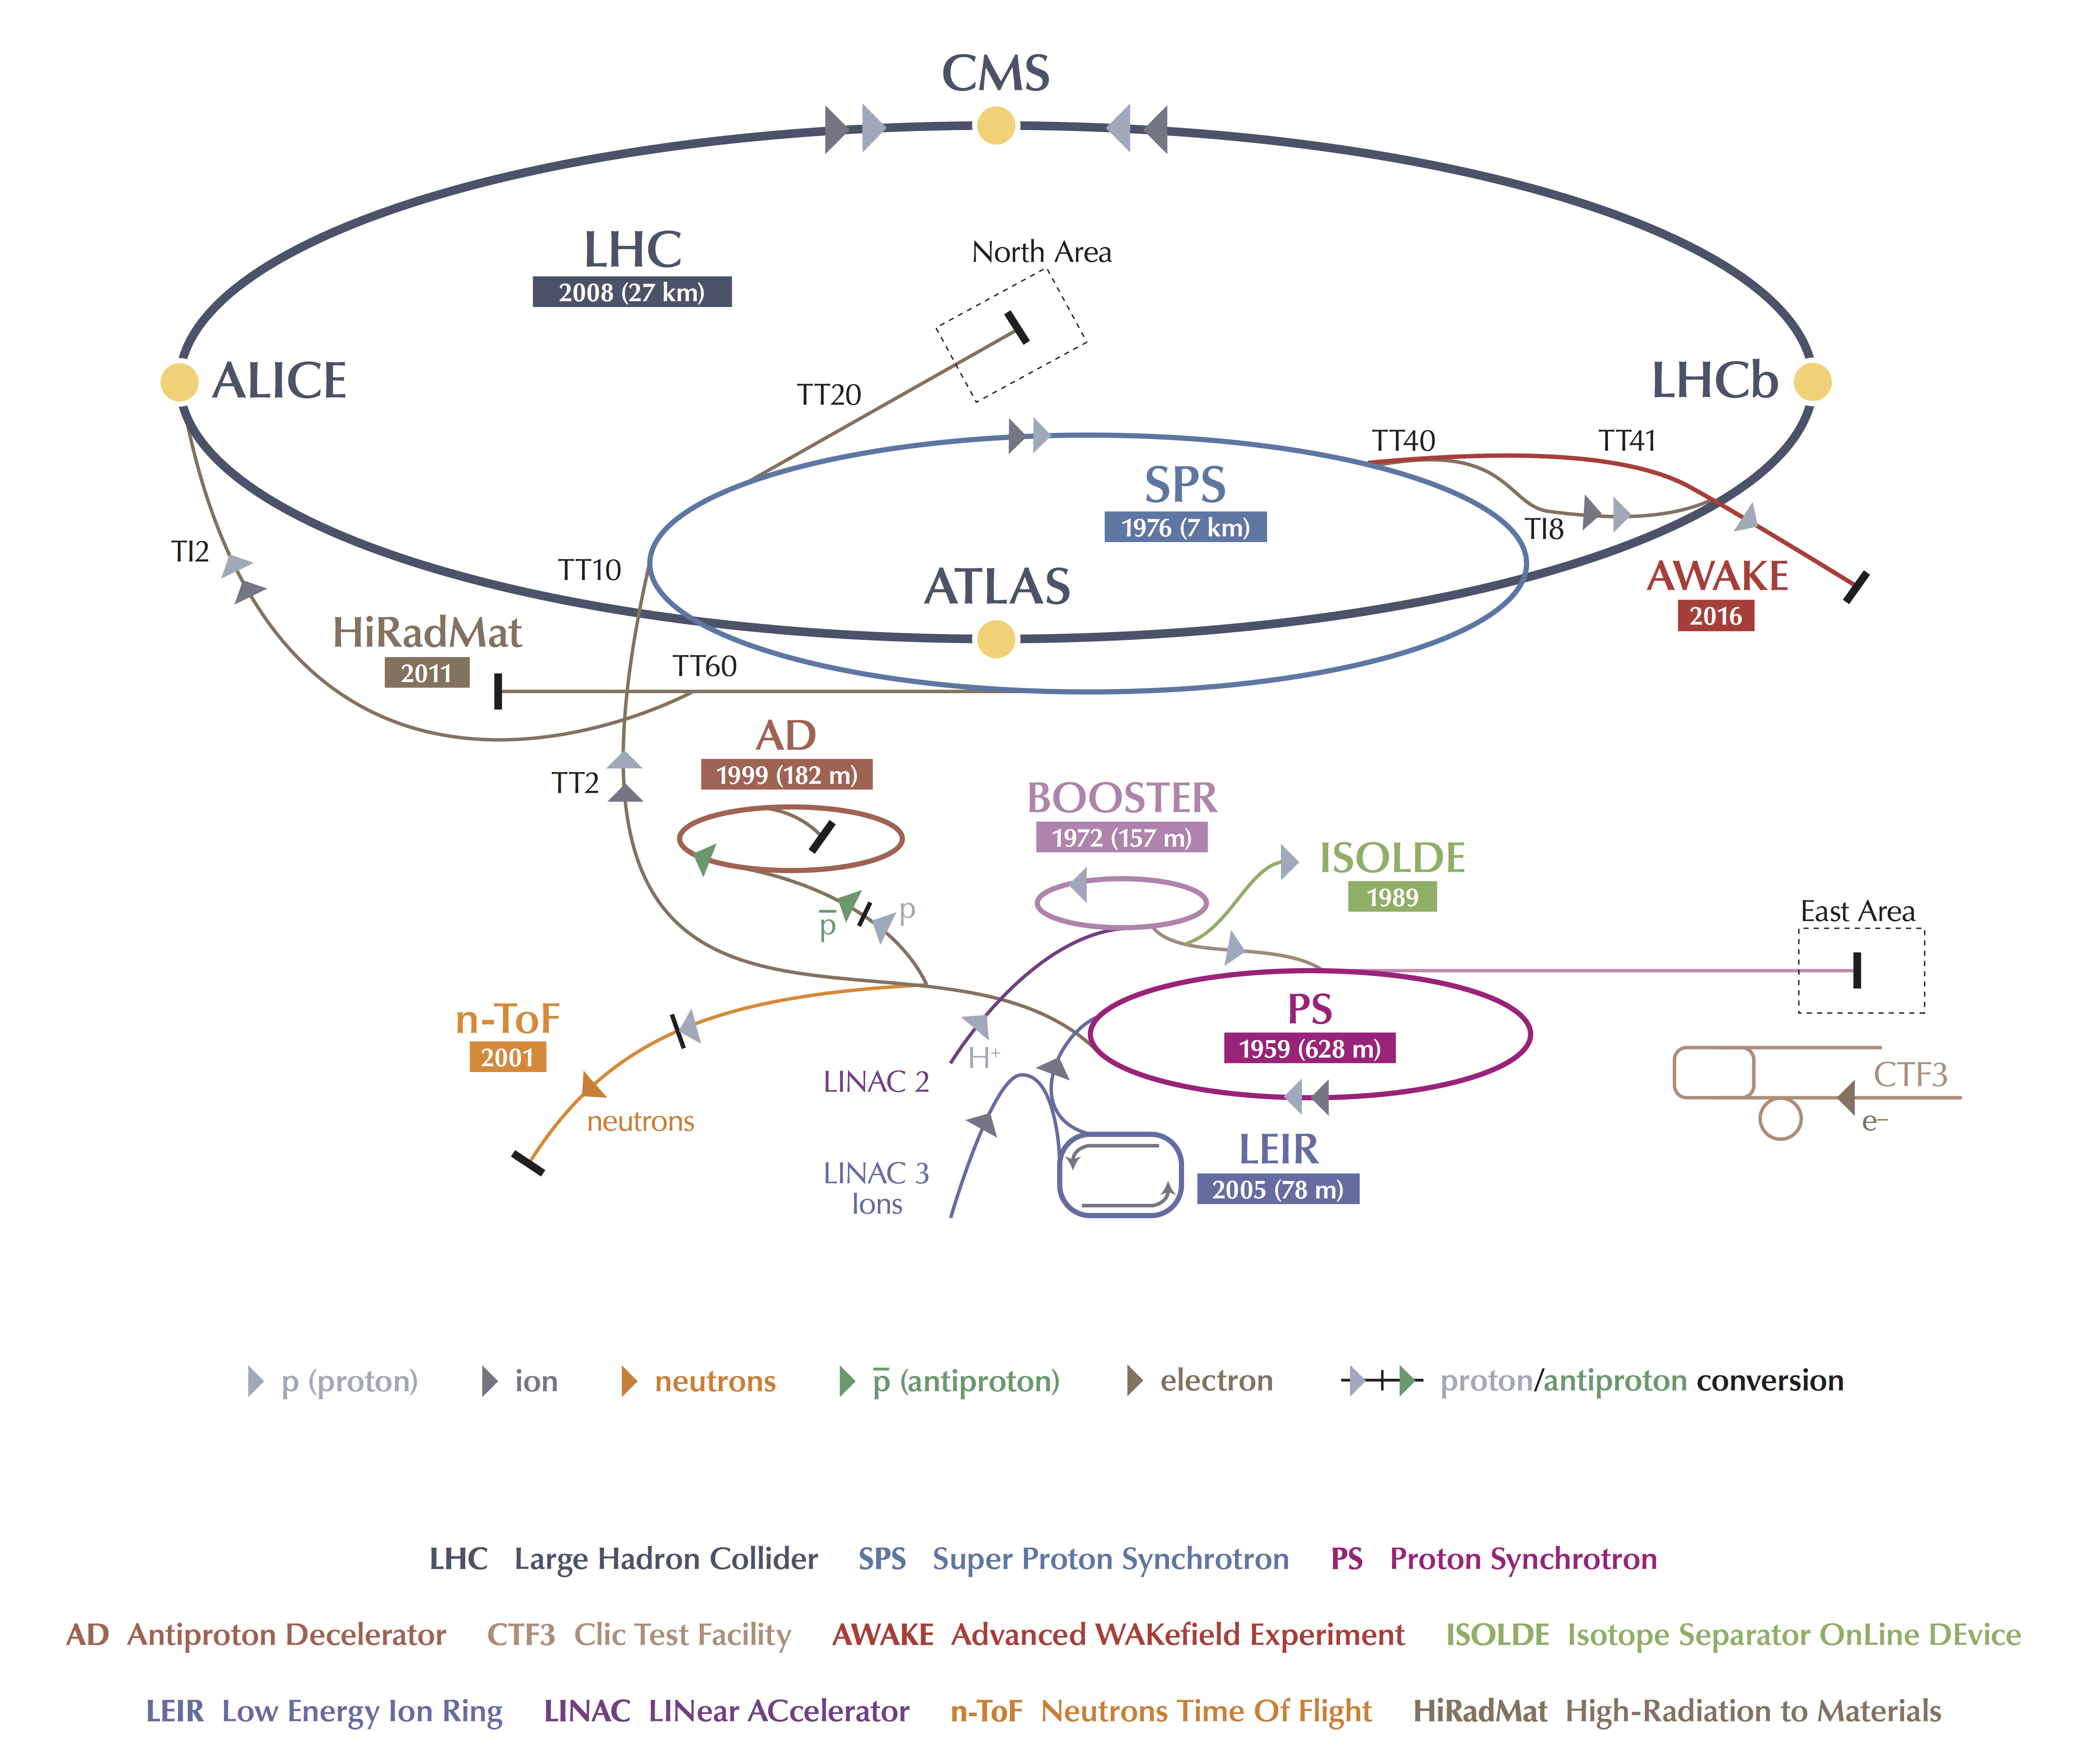
\includegraphics[width=\linewidth]{Figures/LHC/accelerator.jpg}
       \caption{Schematic of the CERN accelerator complex. The LHC is shown in dark grey and includes four interaction points: one each for the CMS, ATLAS, LHCb, and ALICE experiments. Prior to being injected into the LHC, the protons are accelerated through the Linear Accelerator 2 (Linac 2), the Proton Synchrotron Booster, the Proton Synchrotron (PS), and the Super Proton Synchrotron (SPS). Reprinted from Reference~\cite{CDS}.}
       \label{fig:accelerator}
\end{figure*}

\section{LHC tunnel and magnets}
\label{sec:tunnel}

Due to the prohibitive cost of building a new tunnel, the LHC uses the same tunnel as the one previously occupied by the Large Electron-Positron (LEP) Collider. This placed several constraints on the design of the accelerator. Because of the large synchrotron radiation losses that occur when accelerating light particles such as electrons, the LEP tunnel included eight straight sections where the electrons and positrons could be accelerated. For a hadron collider such as the LHC, however, the losses due to synchrotron radiation are less than 7 keV per rotation. The straight sections of the tunnel mean that the arced sections have a smaller radius of curvature $R$ than if the tunnel was perfectly circular. This directly affects the maximum attainable momentum $p$ of a particle with charge $q$ for a given magnetic field $B$:
\begin{equation}
B = \frac{p}{qcR}
\end{equation}

To reach the design energy $\sqrt{s} = 14$ TeV, the LHC dipoles must be able to operate at a magnetic field $B = 8.33$ T. This requires the magnets to be superconducting. The LHC includes 1232 dipole magnets that are cooled to 1.9 K using liquid helium. The magnets are made of stacked niobium-titanium (NbTi) filaments of thickness 6-7 $\mu$m. The LEP tunnel is too narrow (3.7 m radius) to fit two magnet systems and the associated cryogenics and insulation. Therefore, the LHC magnets use a ``twin-bore" design, where both of the beams are embedded in a single magnet system.

The LHC has only one accelerating sector. In the sector, there are eight superconducting RF cavities per beam that operate at a frequency of 400 MHz. The RF cavities increase the energy of the protons by 485 keV per rotation. The beams consist of ``bunches" of protons with a spacing of 25 ns separating consecutive bunches. Each collision between two bunches is referred to as a bunch crossing. 

\section{Machine luminosity}
\label{sec:tunnel}

The number of events $N_{\mathrm{event}}$ produced every second for a particular process with cross section $\sigma_{\mathrm{event}}$ is given by
\begin{equation}
N_{\mathrm{event}} = L\sigma_{\mathrm{event}}
\end{equation}
where $L$ is the instantaneous luminosity of the collider. 

The instantaneous luminosity depends only on machine parameters: 
\begin{equation}
L = \frac{N_b^2 n_b f_{rev} \gamma_r}{4\pi\epsilon_n\beta\ast}F
\end{equation}
The variables in the above equation include the number of particles per bunch $N_b$, the number of bunches per beam $n_b$, the revolution frequency $f_{rev}$, and the relativistic factor $\gamma_r$. For the LHC, $n_b$ is 2808 for the nominal bunch spacing of 25 ns. The number of protons per bunch $N_b$ is limited to 1.15$\times 10^{11}$ by the nonlinear beam-beam interactions between protons at each IP. 

The normalized transverse beam emittance $\epsilon_n$ is a measure of the average spread of particles in the beam in position-momentum phase space. In the transverse direction the beam is assumed to have a Gaussian shape with width $\sigma$. The beta function is then given by $\beta = \sigma^2 /\epsilon$, and $\beta\ast$ refers to the value of the beta function at the interaction point. Finally, $F$ is a geometric factor that depends on the crossing angle at the IP. 

The design instantaneous luminosity of the LHC is 10$^{34}$ cm$^{-2}$ s$^{-1}$. This goal is only attainable because the LHC is a $p$-$p$ collider, rather than a $p$-$\bar{p}$ collider. During the 2016 data-taking period, the LHC met and surpassed its luminosity target, achieving a maximum value of 1.53$\times 10^{34}$ cm$^{-2}$ s$^{-1}$. This is almost double the maximum value of 7.7 $\times 10^{33}$ cm$^{-2}$ s$^{-1}$ that was achieved during Run I. The peak luminosity per day in 2016 is shown in Figure~\ref{fig:instLumi}. The measurement of instantaneous luminosity is described in more detail in Section~\ref{sec:lumi}. 

\begin{figure*}[h!]
	\centering
	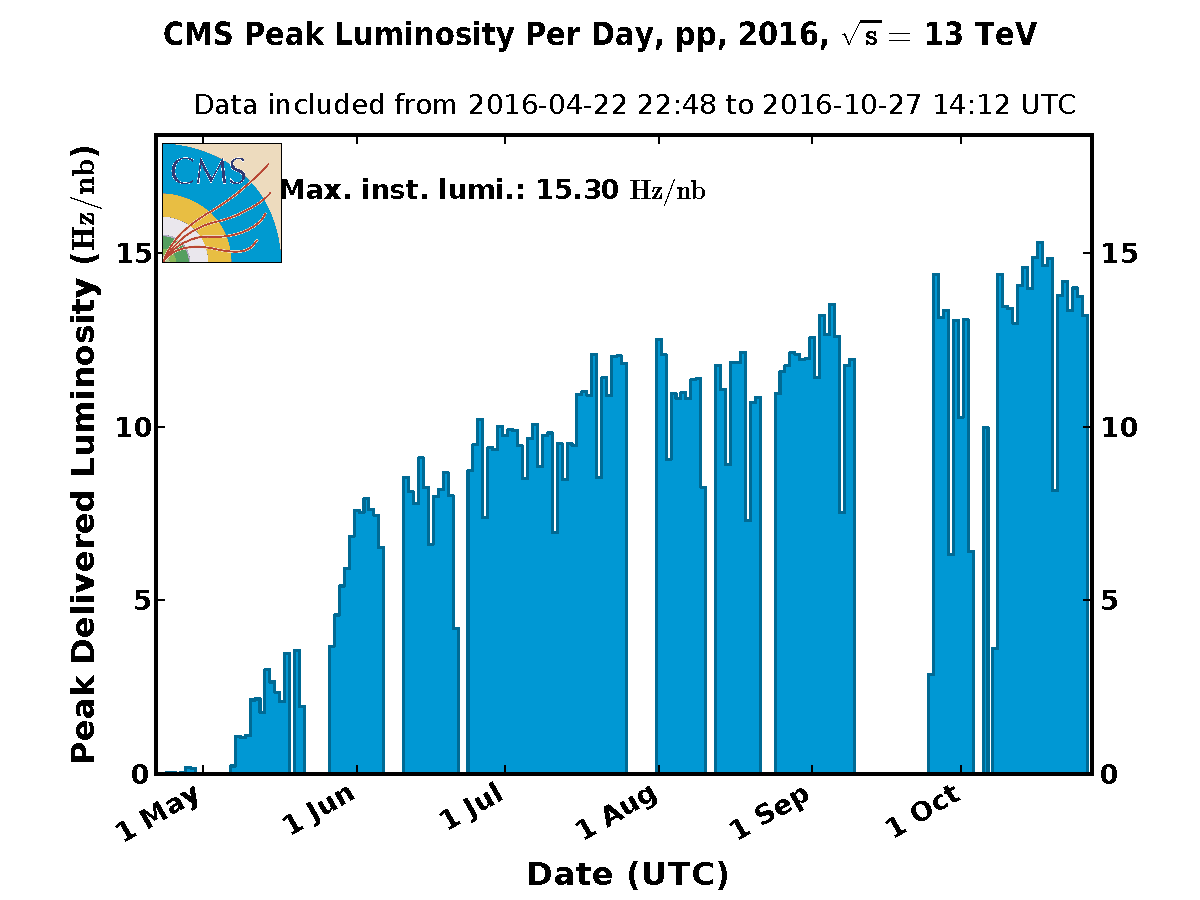
\includegraphics[width=\linewidth]{Figures/LHC/peak_lumi_per_day_pp_2016.pdf}
       \caption{Peak instantaneous luminosity per day achieved by the LHC during the 2016 data-taking period. 
       The maximum luminosity was 15.3 Hz/nb, or 1.53$\times 10^{34}$ cm$^{-2}$ s$^{-1}$. }
       \label{fig:instLumi}
\end{figure*}


%20 minutes to ramp the magnets down after abort
%Minimum LHC injection time is 16 minutes for PS into SPS into LHC
%20 minutes to make sure everything is okay.
%20 minutes to ramp back up

%Improvements between Run I and Run II: 
%https://press.cern/backgrounders/stronger-machine

%Three vacuum systems: 
%insulation vacuum for cryostat, insulation vacuum for helium,  10$^{-1}$ mb
%beam vacuum: more important. Affects beam lifetime (how long one fill lasts) and background from protons scattering off other nonsense in the beam. Must be better than $10^{-10}$ mb at room temp
%"below 1015H2m?3 at cryogenic temperatures (expressed as a gas density normalized to hydrogen, taking into account the ionization cross sections for each gas species)."

